%%%%%%%% ICML 2026 SUBMISSION %%%%%%%%%%%%%%%%%

\documentclass{article}

\usepackage{microtype}
\usepackage{graphicx}
\usepackage{subcaption}
\usepackage{booktabs}
\usepackage{hyperref}

\newcommand{\theHalgorithm}{\arabic{algorithm}}

% For preprint (non-anonymous):
\usepackage[preprint]{icml2026}

\usepackage{amsmath}
\usepackage{amssymb}
\usepackage{mathtools}
\usepackage{amsthm}
\usepackage{multirow}
\usepackage{enumitem}

\icmltitlerunning{Behavioral Consistency in LLM-Based Agents}

\begin{document}

\twocolumn[
  \icmltitle{When Agents Disagree With Themselves: \\ Measuring Behavioral Consistency in LLM-Based Agents}

  \begin{icmlauthorlist}
    \icmlauthor{Aman Mehta}{snow}
  \end{icmlauthorlist}

  \icmlaffiliation{snow}{Snowflake AI Research}

  \icmlcorrespondingauthor{Aman Mehta}{aman.mehta@snowflake.com}
  \icmlkeywords{LLM agents, behavioral consistency, ReAct, reliability, variance}

  \vskip 0.3in
]

\printAffiliationsAndNotice{}

% ============================================================================
% ABSTRACT
% ============================================================================
\begin{abstract}
Run the same LLM agent on the same task twice: do you get the same behavior?
We find the answer is often no.
In a study of 8,000 agent runs across four models and four providers on 200 HotpotQA questions, ReAct-style agents produce 2.3--4.2 distinct action sequences per 10 runs on average.
This variance is associated with failure: consistent tasks ($\leq$2 unique paths) achieve 82--87\% accuracy while inconsistent tasks ($\geq$4 paths) achieve 41--65\%, a gap that persists after controlling for task difficulty (partial $r=-0.16$ to $-0.49$, $p<0.03$).
Divergence concentrates at step~2 (50.5\% of Llama tasks), and consistency metrics achieve AUROC 0.62--0.78 as a lightweight failure detector.
Exploiting this signal, selective prediction---answering only when $k\!=\!3$ runs agree---achieves 87--88\% accuracy at 54--62\% coverage, a 6--14pp improvement over single-run baselines.
A cross-benchmark pilot on SWE-bench (150 runs) preserves the consistency hierarchy, and bootstrap analysis shows single-run evaluations produce incorrect model rankings 29.3\% of the time.
Our results suggest that multi-run evaluation and consistency monitoring should become standard practice for agent deployments.
\end{abstract}

% ============================================================================
% INTRODUCTION
% ============================================================================
\section{Introduction}
\label{sec:intro}

Large language model (LLM) based agents that use tools and multi-step reasoning are increasingly deployed for complex tasks \citep{yao2022react, schick2023toolformer}. As these systems move from prototypes to production, understanding their reliability becomes critical.

A fundamental but understudied question is: \emph{how consistent are LLM agents in their behavior?} Given identical inputs, will an agent follow the same reasoning path and arrive at the same answer? This matters because inconsistency complicates debugging, may signal uncertainty exploitable for error detection, and could inform architecture decisions.

We present a systematic empirical study of behavioral consistency in ReAct-style agents \citep{yao2022react}. Our key contributions:

\begin{enumerate}
    \item \textbf{Quantified behavioral variance}: 8,000 runs (200 tasks $\times$ 10 runs $\times$ 4 models) reveal 2.3--4.2 unique action sequences per task on average.

    \item \textbf{Consistency--correctness association}: Consistent tasks achieve 82--87\% accuracy vs.\ 41--65\% for inconsistent tasks, with effect sizes $r=-0.35$ to $-0.61$ ($p<0.001$) that hold after controlling for task difficulty (partial $r=-0.16$ to $-0.49$).

    \item \textbf{Failure detection}: Consistency metrics achieve AUROC 0.62--0.78 as a runtime failure signal, with precision up to 72\% vs.\ an 18--28\% baseline.

    \item \textbf{Actionable intervention}: Selective prediction via unanimous $k\!=\!3$ agreement achieves 87--88\% accuracy (6--14pp above baselines) at 54--62\% coverage, instantiating the selective classification framework for agents.

    \item \textbf{Early divergence and path length}: 18.8\% of tasks diverge by step~2 (50.5\% for Llama); path length correlates with both consistency and correctness ($\rho=0.50$--$0.74$).

    \item \textbf{Ranking instability}: Single-run evaluations produce incorrect model rankings 29.3\% [28.4--30.1\%] of the time, undermining standard benchmark methodology.
\end{enumerate}

% ============================================================================
% RELATED WORK
% ============================================================================
\section{Related Work}

\paragraph{LLM-Based Agents.}
ReAct \citep{yao2022react} introduced interleaving reasoning with actions. Subsequent work extended this to web browsing \citep{zhou2023webarena}, code execution \citep{yang2024swe}, and multi-agent systems \citep{wu2023autogen}. We study reliability under repeated execution.

\paragraph{Agent Consistency.}
$\tau$-bench \citep{yao2024tau} showed that GPT-4o's pass rate drops from 60\% (pass$^1$) to 25\% (pass$^8$). While $\tau$-bench quantifies \emph{whether} agents are inconsistent, we investigate \emph{where} and \emph{why}: tracing divergence to step~2, correlating consistency with correctness, and identifying path length as a signal. \citet{stroebl2024agents} argue that benchmarks overestimate agent capabilities; our findings support this.

\paragraph{Uncertainty and Selective Prediction.}
Our work connects to three threads. First, \emph{ensemble disagreement}: deep ensembles use prediction variance as an uncertainty estimate \citep{lakshminarayanan2017simple}; behavioral consistency across agent runs is an analogous signal, where each run acts as an implicit ensemble member. Second, \emph{self-consistency}: \citet{wang2022self} show that majority voting over sampled reasoning chains improves accuracy; we extend this from single-turn CoT to multi-step agentic settings and additionally study consistency as a \emph{diagnostic} signal, not just an ensembling strategy (Section~\ref{sec:intervention}). Third, \emph{selective prediction}: \citet{geifman2017selective} and \citet{kamath2020selective} show that abstaining on uncertain inputs improves precision; our consistency-filtered results instantiate this for agents. Unlike verbalized confidence \citep{xiong2024llms, tian2023just}, behavioral consistency requires no model modification---it emerges naturally from repeated execution. Prior work on LLM calibration \citep{kadavath2022language} and semantic uncertainty \citep{kuhn2023semantic} focuses on single-turn outputs; we extend to multi-step agentic behavior.

% ============================================================================
% METHODOLOGY
% ============================================================================
\section{Methodology}

\subsection{Agent Architecture}

We implement a ReAct-style agent with three tools: \textbf{Search(query)} returns document titles via keyword matching, \textbf{Retrieve(title)} returns full text, and \textbf{Finish(answer)} terminates with a final answer. The agent follows the standard think--act--observe loop.

\subsection{Experimental Setup}

\paragraph{Dataset.} We use 200 questions from HotpotQA \citep{yang2018hotpotqa} validation (distractor setting), requiring multi-hop reasoning over 10 paragraphs (2 gold, 8 distractors).

\paragraph{Models.} Four models across four providers: Llama 3.1 70B (Meta), GPT-5 (OpenAI), Claude Sonnet 4.5 (Anthropic), and Gemini 3 Pro (Google). We additionally report GPT-4o results on a 100-question subset in Appendix~\ref{app:gpt4o}.

\paragraph{Runs.} For each question--model pair, 10 independent runs at temperature 0.7, yielding 8,000 total runs. Gemini 3 Pro required an additional \texttt{top\_p\,=\,0.95} parameter to achieve stochastic sampling (Appendix~\ref{sec:gemini_note}). Temperature ablation: 20 questions $\times$ 5 runs $\times$ 4 models $\times$ 3 temperatures.

\paragraph{Statistical note.} All tests are two-sided; raw $p$-values without multiple-comparison correction given the exploratory nature.

\subsection{Metrics}

\textbf{Answer consistency}: fraction of runs producing the most common answer. \textbf{Action sequence diversity}: number of unique action sequences across $N$ runs. \textbf{Step variance ratio}: $(\max - \min)/\text{mean}$ of step counts. \textbf{First divergence point}: earliest step where runs take different actions. \textbf{Correctness}: fuzzy string matching (answer contains gold or vice versa, case-insensitive); results under exact match and token F1 in Appendix~\ref{app:metrics}.

% ============================================================================
% RESULTS
% ============================================================================
\section{Results}

\begin{figure*}[t]
\centering
\begin{subfigure}[t]{0.48\textwidth}
\centering

\includegraphics[width=\textwidth]{unique_sequences_histogram.png}
\caption{Distribution of unique action sequences per task.}
\label{fig:histogram}
\end{subfigure}
\hfill
\begin{subfigure}[t]{0.48\textwidth}
\centering

\includegraphics[width=\textwidth]{correctness_comparison.png}
\caption{Correctness for consistent ($\leq$2 seqs) vs.\ inconsistent ($\geq$4 seqs) tasks.}
\label{fig:correctness}
\end{subfigure}
\caption{Behavioral consistency varies across models (left) and is associated with correctness (right).}
\label{fig:main}
\end{figure*}

\subsection{Overall Model Comparison}

Table~\ref{tab:overall} summarizes 8,000 runs. Claude Sonnet 4.5 achieves both the highest accuracy and consistency (2.3 unique sequences). Llama 3.1 70B shows the most behavioral variance (4.2 unique sequences), followed by Gemini 3 Pro (3.2). All four models exhibit measurable behavioral inconsistency even on identical inputs.

\begin{table}[h]
\centering
\small
\caption{Performance across four models (200 tasks each). Seqs = unique action sequences; Var = step variance ratio.}
\label{tab:overall}
\begin{tabular}{lcccc}
\toprule
\textbf{Model} & \textbf{Correct} & \textbf{Seqs} & \textbf{Steps} & \textbf{Var} \\
\midrule
Claude Sonnet 4.5 & \textbf{81.5\%} & \textbf{2.3} & 5.1 & \textbf{22.2\%} \\
GPT-5 & 79.6\% & 2.4 & 4.2 & 36.0\% \\
Llama 3.1 70B & 73.7\% & 4.2 & 4.7 & 64.9\% \\
Gemini 3 Pro & 72.2\% & 3.2 & 5.4 & 38.5\% \\
\bottomrule
\end{tabular}
\end{table}

\subsection{Consistency Is Associated with Correctness}

Table~\ref{tab:consistency} shows the central finding: consistent tasks ($\leq$2 unique sequences) achieve 82--87\% accuracy while inconsistent tasks ($\geq$4 sequences) achieve 41--65\%. The gap is significant for all four models (Mann-Whitney $U$, all $p<0.001$; rank-biserial $r=-0.35$ to $-0.61$).

\begin{table}[h]
\centering
\small
\caption{Correctness (\%) by consistency level. Gap in pp. $r$ = rank-biserial; $n$ = consistent/inconsistent counts. All $p<0.001$.}
\label{tab:consistency}
\begin{tabular}{l@{\hskip 4pt}c@{\hskip 4pt}c@{\hskip 4pt}c@{\hskip 4pt}c@{\hskip 4pt}c}
\toprule
\textbf{Model} & \textbf{Cons.} & \textbf{Incons.} & \textbf{Gap} & \textbf{$r$} & \textbf{$n$} \\
 & ($\leq$2) & ($\geq$4) & & & \\
\midrule
Gemini 3 Pro & 86.5 & 41.2 & 45.3 & $-$.61 & 122/66 \\
GPT-5 & 85.9 & 53.1 & 32.8 & $-$.43 & 141/29 \\
Claude Son.\ 4.5 & 86.4 & 60.3 & 26.1 & $-$.39 & 155/32 \\
Llama 70B & 82.3 & 64.7 & 17.6 & $-$.35 & 61/104 \\
\bottomrule
\end{tabular}
\end{table}

\paragraph{Controlling for difficulty.} Task difficulty confounds the consistency--correctness relationship. We compute a difficulty proxy (mean correctness across all models) and bin questions into Easy ($\geq$0.80, $n=132$), Medium (0.40--0.79, $n=32$), and Hard ($<$0.40, $n=36$). Within Easy tasks, the consistency gap is positive for Gemini ($+$16.5pp) and Llama ($+$11.2pp) but near zero for Claude and GPT-5, reflecting ceiling effects where both consistent and inconsistent Easy tasks achieve $>$90\% accuracy. Within Medium tasks, the gap is positive for all four models ($+$7 to $+$34pp), though cell sizes are small ($n_c$=6--16, $n_i$=10--22; Appendix~\ref{app:difficulty}). For Hard tasks, the gap reverses for three of four models under fuzzy match. This reversal is a \emph{consistent-wrong} phenomenon: of 61 consistent Hard task-model pairs, 52 (85.2\%) are scored incorrect under fuzzy match. Approximately 30\% of these are false negatives---surface-form mismatches where the model produced a semantically correct answer (e.g., ``Pasek and Paul'' vs.\ gold ``Pasek \& Paul''; ``Kelly Osbourne'' vs.\ ``Kelly Lee Osbourne''). Annotation protocol: the author classified each case as surface-form mismatch vs.\ genuinely incorrect; all annotated cases and classification criteria are available in the repository. When we recompute Hard stratum gaps under token F1 $\geq$ 0.5, all four models show non-negative gaps ($+$0 to $+$16pp; Table~\ref{tab:f1_hard}), confirming that the reversal is a fuzzy-match artifact. The remaining $\sim$70\% represent true consistent-wrong behavior, where the agent confidently commits to a wrong answer. Full analysis in Appendix~\ref{app:difficulty}. The within-stratum association is weaker than the aggregate effect, consistent with difficulty being the primary confound. Partial correlations (controlling for difficulty as a continuous variable) remain significant for three of four models: Gemini ($r=-0.49$, $p<0.001$), GPT-5 ($r=-0.16$, $p=0.025$), and Llama ($r=-0.16$, $p=0.028$). The non-significant partial correlation for Claude ($r=0.01$, $p=0.88$) reflects a ceiling effect: Claude is consistent-correct on 68\% of tasks, leaving insufficient within-model variance for the partial correlation to detect.

\subsection{Consistency as a Runtime Failure Detector}
\label{sec:failure_detection}

We frame failure detection as binary classification: predicting whether the majority answer is incorrect using only consistency metrics. Table~\ref{tab:detection} reports the best feature per model.

\begin{table}[h]
\centering
\small
\caption{Failure detection via consistency metrics. H = answer entropy. Baseline precision equals the per-model error rate.}
\label{tab:detection}
\begin{tabular}{llccc}
\toprule
\textbf{Model} & \textbf{Feat.} & \textbf{Prec.} & \textbf{Rec.} & \textbf{AUROC} \\
\midrule
Gemini 3 Pro & Seq$>$4 & 72.1\% & 54.4\% & .775 \\
Llama 70B & H$>$1.5 & 44.9\% & 50.0\% & .714 \\
GPT-5 & H$>$1.5 & 35.5\% & 56.4\% & .688 \\
Claude Son.\ 4.5 & H$>$0.5 & 23.9\% & 63.6\% & .619 \\
\bottomrule
\end{tabular}
\end{table}

For the most variable models (Llama, GPT-5, Gemini), consistency metrics achieve AUROC 0.69--0.78, substantially above the 0.50 random baseline. Even for the most consistent model (Claude), AUROC reaches 0.62, validating consistency as a lightweight runtime failure signal across all four models. Gemini's best predictor is unique sequences rather than answer entropy ($>$4 sequences indicates likely failure); with 66 inconsistent tasks in 200 questions, Gemini provides sufficient signal for the sequence-count feature to outperform entropy-based thresholds.

\subsection{Majority Voting and Selective Prediction}
\label{sec:intervention}

Can consistency be \emph{exploited}, not just observed? We simulate a majority-vote intervention using existing multi-run data: for budget $k$, subsample $k$ runs per question, take the majority answer, and evaluate accuracy (500 bootstrap iterations).

\begin{table}[h]
\centering
\small
\caption{Majority-vote accuracy (\%) and selective prediction. $k\!=\!1$ is single-run baseline. Sel.\ = unanimous $k\!=\!3$ (answer only when all 3 agree).}
\label{tab:vote}
\begin{tabular}{l@{\hskip 5pt}c@{\hskip 5pt}c@{\hskip 5pt}c@{\hskip 5pt}c@{\hskip 5pt}c}
\toprule
\textbf{Model} & $k\!=\!1$ & $k\!=\!3$ & \textbf{Gain} & \textbf{Sel.\ Acc} & \textbf{Cov.} \\
\midrule
Llama 70B & 73.6 & 75.6 & +2.0 & 87.2 & 53.8 \\
Claude Son.\ 4.5 & 81.5 & 82.2 & +0.7 & 87.8 & 61.8 \\
GPT-5 & 79.6 & 80.1 & +0.5 & 88.1 & 55.2 \\
Gemini 3 Pro & 72.2 & 72.3 & $+$0.1 & 73.3 & 64.9 \\
\bottomrule
\end{tabular}
\end{table}

Table~\ref{tab:vote} reveals that consistency works far better as a \emph{filter} than an \emph{aggregator}---a striking contrast with single-turn self-consistency \citep{wang2022self}, where majority voting improves CoT accuracy by 5--17pp. In our multi-step agentic setting, voting yields only +0--2pp because agentic errors are \emph{systematic}: an early wrong action commits the agent to an incorrect trajectory, producing consistent-wrong answers that voting cannot correct. \emph{Selective prediction}---answering only when all $k\!=\!3$ runs agree---is the stronger intervention: for Llama, Claude, and GPT-5, unanimous agreement achieves 87--88\% accuracy (6--14pp above baselines) at 54--62\% coverage. The asymmetry is explained by a 2$\times$2 taxonomy of task outcomes: consistent-correct tasks (25--68\% per model) are retained; inconsistent-wrong tasks (6--19\%) are filtered; the ceiling is set by \emph{consistent-wrong} tasks (5--10\%), where the model confidently errs. Notably, 61\% of Claude's errors are consistent-wrong vs.\ only 25\% of Llama's, explaining why Llama benefits most from voting. Stricter thresholds yield further gains: unanimous 5/5 agreement achieves 90.2\% accuracy for GPT-5 at 48\% coverage (full taxonomy and thresholds in Appendix~\ref{app:vote}).

\subsection{Divergence Occurs Early; Path Length Matters}

Pooled across four models, 18.8\% [95\% CI: 16.2--21.6\%] of tasks diverge by step~2, but this rate varies dramatically: Llama diverges early in 50.5\% [43.6--57.4\%] of tasks vs.\ 4--6\% for Claude and GPT-5. Among Llama's early-diverging tasks, accuracy is 71.7\% vs.\ 85.8\% for late-diverging tasks. The first search query largely determines the trajectory.

Path length correlates with both consistency and correctness: Spearman $\rho$ between mean steps and unique sequences is 0.74 (Llama), 0.54 (Gemini), 0.53 (Claude), 0.50 (GPT-5); pooled $\rho=0.51$, all $p<0.001$. Longer paths indicate backtracking and uncertainty; each additional step is an opportunity to diverge and err.

\subsection{Temperature Ablation}

Figure~\ref{fig:temp} shows results across all four models. All models show monotonically increasing unique sequences with temperature. Claude and Gemini achieve near-perfect consistency at $T\!=\!0.0$ (1.0 sequences) while Llama retains 2.3, suggesting that model architecture matters beyond sampling noise. The accuracy--temperature tradeoff is model-dependent: GPT-5 and Llama show minimal accuracy change across temperatures. The finding that $T\!=\!0.0$ does not eliminate divergence for Llama or GPT-5 indicates that agentic inconsistency arises from factors beyond token-level sampling. Full table in Appendix~\ref{app:temp}.

\begin{figure}[h]
\centering
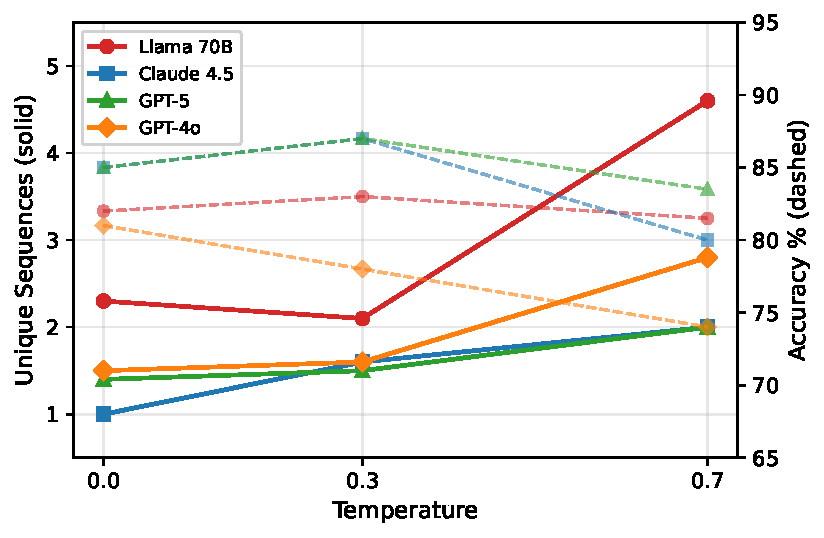
\includegraphics[width=\columnwidth]{temperature_ablation.pdf}
\caption{Temperature ablation (20 questions, 5 runs). Solid: unique sequences (left axis); dashed: accuracy (right axis).}
\label{fig:temp}
\end{figure}

\subsection{Cross-Benchmark Pilot: SWE-bench}
\label{sec:swebench}

To test generalizability beyond HotpotQA's minimal action space, we conduct a pilot study on SWE-bench Verified \citep{swebench, swebench_verified}: 10 astropy tasks, 5 runs per model-task pair (150 runs), using three of our four HotpotQA models---Claude, GPT-5, and Llama---with an identical bash-only scaffold (temperature 0.5).

\begin{table}[h]
\centering
\small
\caption{SWE-bench pilot (10 tasks $\times$ 5 runs). CV = std/mean of step counts. The HotpotQA consistency hierarchy is preserved.}
\label{tab:swebench}
\begin{tabular}{lccc}
\toprule
& \textbf{Claude} & \textbf{GPT-5} & \textbf{Llama} \\
\midrule
CV & \textbf{15.2\%} & 32.2\% & 47.0\% \\
Accuracy & \textbf{58\%} & 32\% & 4\% \\
Unique Seqs & 100\% & 100\% & 100\% \\
\bottomrule
\end{tabular}
\end{table}

The consistency ranking is identical to HotpotQA (Claude $>$ GPT-5 $>$ Llama), consistent with consistency being a stable model-level property. All 150 runs produced unique action sequences, yet CV still discriminates between models. The accuracy gap widens from 8pp (HotpotQA) to 54pp (SWE-bench), consistent with the hypothesis that complexity amplifies consistency effects. Given the small sample (10 tasks, single repository), these results are preliminary; full cross-benchmark comparison in Appendix~\ref{app:swebench}.

\subsection{Ranking Instability}
\label{sec:rankings}

We perform 10,000 bootstrap iterations across four models on all 200 questions, sampling one run per question per model. \textbf{29.3\% [28.4--30.1\%] of single-run evaluations produce a ranking differing from the multi-run ground truth} (Claude 81.5\% $>$ GPT-5 79.6\% $>$ Llama 73.7\% $>$ Gemini 72.2\%). Nearly one in three single-run evaluations would misrank models. The instability stems from narrow accuracy gaps between adjacent models and within-model variance. Agent benchmarks should report multi-run statistics.

% ============================================================================
% DISCUSSION
% ============================================================================
\section{Discussion}

\paragraph{Beyond $\tau$-bench.}
While $\tau$-bench \citep{yao2024tau} established that agents are inconsistent, we provide complementary insights: \emph{where} variance originates (step~2), its association with correctness ($r=-0.35$ to $-0.61$), and its practical utility for failure detection (AUROC 0.62--0.78). These findings suggest actionable interventions beyond measuring pass$^k$.

\paragraph{Practical implications.}
Consistency monitoring is feasible and actionable. Our majority-vote experiment (Section~\ref{sec:intervention}) shows that even $k\!=\!3$ runs suffice: selective prediction on unanimous agreement achieves 87--88\% accuracy for three models, a 6--14pp gain over single-run baselines at 54--62\% coverage. Crucially, consistency functions as a \emph{filter} (abstain on disagreement) rather than an \emph{aggregator} (vote to pick the best): voting gains are minimal (+0--2pp), but filtering gains are substantial (+4--13pp). The ceiling on filtering is set by consistent-wrong tasks (5--13\% per model), where the agent confidently commits to an incorrect answer. Consistency metrics provide a complementary lightweight signal (AUROC 0.62--0.78). The step~2 bottleneck suggests that improving first-query formulation could reduce downstream variance.

\paragraph{Consistency as implicit calibration.}
Traditional calibration asks whether a model's stated confidence matches its accuracy \citep{kadavath2022language}. Behavioral consistency provides an alternative, \emph{behavioral} notion of calibration: agents that produce diverse trajectories across runs are implicitly signaling uncertainty about the task, much as deep-ensemble disagreement signals epistemic uncertainty \citep{lakshminarayanan2017simple}. Unlike verbalized confidence---which requires prompting strategies and is often poorly calibrated \citep{xiong2024llms, tian2023just}---behavioral consistency emerges naturally from repeated execution and requires no model modification. Our selective-prediction results (Table~\ref{tab:vote}) confirm that this implicit signal is actionable: unanimous agreement among $k\!=\!3$ runs selects for high-accuracy subsets. This positions multi-run consistency as a practical calibration mechanism for deployed agents.

\paragraph{Limitations and future work.}
Our analysis primarily uses HotpotQA with a 3-tool action space; the SWE-bench pilot provides preliminary evidence of generalizability. The temperature ablation uses a smaller sample (20 questions). We cannot establish causality from observational data. Gemini 3 Pro required a \texttt{top\_p} workaround to achieve stochastic sampling (Appendix~\ref{sec:gemini_note}). We plan extensions to multimodal agents and analytical reasoning (FinQA, GAIA).

% ============================================================================
% CONCLUSION
% ============================================================================
\section{Conclusion}

Behavioral consistency in LLM agents is measurable, associated with correctness, and practically exploitable. Across 8,000 runs on four models, consistent agents achieve 82--87\% accuracy vs.\ 41--65\% for inconsistent ones, with effect sizes that survive difficulty controls. Consistency metrics detect failures with AUROC 0.62--0.78, and selective prediction on unanimous $k\!=\!3$ agreement yields 87--88\% accuracy at 54--62\% coverage---demonstrating that behavioral consistency functions as an actionable confidence signal. Single-run evaluations produce incorrect rankings 29.3\% of the time. These findings argue for multi-run evaluation, consistency-based selective prediction, and runtime consistency monitoring as standard practice.

Code and data: \url{https://github.com/amanmehta-maniac/agent-consistency}.

% ============================================================================
% IMPACT STATEMENT
% ============================================================================
\section*{Impact Statement}

Our finding that single-run evaluations produce incorrect model rankings 29\% of the time has direct implications for practitioners who rely on benchmark scores to select agent models. For high-stakes deployments, monitoring behavioral consistency across parallel executions could serve as a lightweight failure detection mechanism with AUROC 0.62--0.78. We provide diagnostic tools for understanding existing limitations rather than new capabilities, and do not foresee negative societal consequences from this work.

% ============================================================================
% REFERENCES
% ============================================================================
\bibliography{references}
\bibliographystyle{icml2026}

% ============================================================================
% APPENDIX
% ============================================================================
\appendix

\section{Gemini 3 Pro: Sampling Configuration}
\label{sec:gemini_note}

Gemini 3 Pro on the Snowflake Cortex endpoint initially exhibited near-deterministic outputs at $T\!=\!0.7$, producing identical action sequences in $>$99\% of runs. We determined that the endpoint does not fully respect the \texttt{temperature} parameter without explicitly setting \texttt{top\_p} $< 1.0$. After adding \texttt{top\_p = 0.95}, outputs became properly stochastic (3.2 unique sequences on average, comparable to GPT-5). All Gemini results---including temperature ablation---use the corrected stochastic configuration.

\section{Temperature Ablation: Full Results}
\label{app:temp}

\begin{table}[h]
\centering
\caption{Full temperature ablation (20 questions, 5 runs each). $T\!=\!0.7$ uses same questions from the main experiment.}
\small
\begin{tabular}{llcc}
\toprule
\textbf{Model} & \textbf{Temp} & \textbf{Accuracy} & \textbf{Unique Seqs} \\
\midrule
\multirow{3}{*}{Llama 3.1 70B} & 0.0 & 82.0\% & 2.3 \\
& 0.3 & 83.0\% & 2.1 \\
& 0.7 & 82.0\% & 3.3 \\
\midrule
\multirow{3}{*}{Claude Sonnet 4.5} & 0.0 & 85.0\% & 1.0 \\
& 0.3 & 87.0\% & 1.6 \\
& 0.7 & 85.0\% & 1.7 \\
\midrule
\multirow{3}{*}{GPT-5} & 0.0 & 85.0\% & 1.4 \\
& 0.3 & 87.0\% & 1.5 \\
& 0.7 & 87.0\% & 1.6 \\
\midrule
\multirow{3}{*}{Gemini 3 Pro} & 0.0 & 75.0\% & 1.0 \\
& 0.3 & 76.0\% & 2.0 \\
& 0.7 & 75.0\% & 2.2 \\
\bottomrule
\end{tabular}
\end{table}

\section{Difficulty Stratification: Full Results}
\label{app:difficulty}

Task difficulty is computed as mean correctness across all runs from all four models. Strata: Easy ($\geq$0.80), Medium (0.40--0.79), Hard ($<$0.40). Of 200 questions: 132 Easy, 32 Medium, 36 Hard.

\begin{table}[h]
\centering
\small
\caption{Consistency--correctness gap (pp) within difficulty strata. $n_c$/$n_i$ = number of consistent/inconsistent tasks per model in that stratum.}
\scriptsize
\begin{tabular}{lcccc}
\toprule
\textbf{Stratum} & \textbf{Llama} & \textbf{GPT-5} & \textbf{Claude} & \textbf{Gemini} \\
\midrule
Easy (132) & $+$11.2pp & $+$6.8pp & $-$0.5pp & $+$16.5pp \\
 & {\tiny 46/58} & {\tiny 106/8} & {\tiny 119/9} & {\tiny 100/23} \\
Medium (32) & $+$6.7pp & $+$15.0pp & $+$6.4pp & $+$34.3pp \\
 & {\tiny 6/22} & {\tiny 16/10} & {\tiny 16/11} & {\tiny 9/21} \\
Hard (36) & $-$5.6pp & $+$8.9pp & $-$5.8pp & $-$4.2pp \\
 & {\tiny 9/24} & {\tiny 19/11} & {\tiny 20/12} & {\tiny 13/22} \\
\bottomrule
\end{tabular}
\end{table}

Partial correlations between unique sequences and accuracy, controlling for difficulty (continuous): Gemini $r=-0.487$ ($p<0.001$), GPT-5 $r=-0.159$ ($p=0.025$), Llama $r=-0.156$ ($p=0.028$), Claude $r=0.011$ ($p=0.877$). The association remains significant for three of four models.

\paragraph{Consistent-Wrong analysis.} The Hard stratum reversal (negative gaps above) is explained by \emph{consistent-wrong} behavior: on tasks where the model lacks knowledge, consistency reflects confident commitment to an incorrect answer rather than reliable competence. We classify each model$\times$Hard-task pair into four categories based on unique action sequences and correctness:

\begin{itemize}[nosep,leftmargin=*]
  \item \textbf{Consistent-Correct} ($\leq$2 seqs, majority correct): 9/144 (6.3\%)
  \item \textbf{Consistent-Wrong} ($\leq$2 seqs, majority wrong): 52/144 (36.1\%)
  \item \textbf{Inconsistent-Lucky} ($\geq$4 seqs, $\geq$1 correct run): 27/144 (18.8\%)
  \item \textbf{Inconsistent-Wrong} ($\geq$4 seqs, 0 correct): 42/144 (29.2\%)
\end{itemize}

Among consistent Hard tasks, 85.2\% (52/61) are Consistent-Wrong---the model locks into one incorrect reasoning path. Of these, approximately 30\% are false negatives under token F1 $\geq$ 0.5: the model produced a semantically correct answer in a different surface form (e.g., ``Pasek and Paul'' for gold ``Pasek \& Paul'', ``Kelly Osbourne'' for gold ``Kelly Lee Osbourne''). The remaining $\sim$70\% are genuinely incorrect. When recomputed under token F1 $\geq$ 0.5, the Hard reversal disappears: all four models show non-negative consistency gaps ($+$0 to $+$16pp; Table~\ref{tab:f1_hard}), confirming that the consistency--correctness association holds under a more permissive metric. Conversely, 39.1\% (27/69) of inconsistent Hard tasks achieve at least one correct run, confirming that behavioral variability enables exploration that occasionally recovers the right answer. Per-model consistent-wrong rates (fuzzy): Llama 100\% (9/9), GPT-5 79\% (15/19), Claude 80\% (16/20), Gemini 92\% (12/13).

\begin{table}[h]
\centering
\small
\caption{Hard stratum consistency gap (pp) under token F1 $\geq$ 0.5. All gaps are non-negative, confirming the fuzzy-match reversal is a metric artifact.}
\label{tab:f1_hard}
\scriptsize
\begin{tabular}{lcccc}
\toprule
& \textbf{Llama} & \textbf{GPT-5} & \textbf{Claude} & \textbf{Gemini} \\
\midrule
Gap (pp) & $+$8.9 & $+$16.1 & $+$9.7 & $+$11.5 \\
$n_c$/$n_i$ & 9/24 & 19/11 & 20/12 & 13/22 \\
\bottomrule
\end{tabular}
\end{table}

\section{Cross-Benchmark Comparison}
\label{app:swebench}

\begin{table}[h]
\centering
\small
\caption{HotpotQA vs.\ SWE-bench. Consistency ranking preserved; accuracy gaps widen with task complexity.}
\begin{tabular}{lcc}
\toprule
& \textbf{HotpotQA} & \textbf{SWE-bench} \\
\midrule
Action space & 3 tools & Unrestricted bash \\
Avg trajectory & 3--8 steps & 10--46 steps \\
Best model CV & 8.2\% (Claude) & 15.2\% (Claude) \\
Worst model CV & 22.1\% (Llama) & 47.0\% (Llama) \\
Accuracy range & 73--82\% & 4--58\% \\
Mean unique seqs & 2.3--4.2 & all unique \\
Ranking preserved & \multicolumn{2}{c}{$\checkmark$ (Claude $>$ GPT $>$ Llama)} \\
\bottomrule
\end{tabular}
\end{table}

\section{GPT-4o: Additional Validation on 100-Question Subset}
\label{app:gpt4o}

We additionally evaluated GPT-4o (OpenAI) on a 100-question subset (questions 1--100) collected when the model was available via our API provider. Results are consistent with the main findings: GPT-4o shows 2.5 unique sequences per task (comparable to GPT-5's 2.4), 73.3\% accuracy, and a consistency--correctness gap of 35.9pp ($r=-0.47$, $p<0.001$). Failure detection achieves AUROC 0.661, and the path length correlation is $\rho=0.43$ ($p<0.001$). Temperature ablation shows GPT-4o gains $+$9pp accuracy at $T\!=\!0.0$, the largest temperature effect observed across all models tested. These results confirm that the consistency hierarchy extends to earlier-generation frontier models and that our findings are not specific to the four primary models in the main text.

\section{Question Type Analysis}
\label{app:qtype}

On the first 100 questions with type annotations, we compare bridge questions (multi-hop, $n=79$) with comparison questions (yes/no, $n=21$) using Llama 3.1 70B. Comparison questions show \emph{higher} correctness (80.0\% vs.\ 75.7\%) but \emph{lower} answer consistency (62.4\% vs.\ 76.6\%) and lower step variance (41\% vs.\ 63\%), highlighting that answer consistency and explanation consistency are distinct dimensions.

\section{Metric Sensitivity}
\label{app:metrics}

We verify robustness to the choice of correctness metric. Under exact match (EM), overall accuracy decreases (e.g., Claude: 43.6\% EM vs.\ 81.5\% fuzzy) but model rankings and consistency gaps are preserved. Under token F1 $>$ 0.5, results closely track fuzzy match. The consistency--correctness association holds across all three metrics for all four models.

\section{Majority Voting and Selective Prediction: Full Results}
\label{app:vote}

\paragraph{Task-outcome taxonomy.} Table~\ref{tab:taxonomy} classifies each task by consistency ($\leq$2 vs.\ $\geq$4 unique sequences) and correctness (majority answer matches gold). The taxonomy explains why filtering outperforms voting: consistent-wrong tasks (5--13\%) set the ceiling on filtering, while inconsistent-correct tasks (8--38\%)---where voting could theoretically consolidate the right answer---are rare except for Llama.

\begin{table}[h]
\centering
\small
\caption{Task-outcome taxonomy (\% of tasks). Consistent: $\leq$2 unique seqs; Inconsistent: $\geq$4. Rows sum to $<$100\% because tasks with exactly 3 unique sequences (6--17\% per model) fall between thresholds.}
\label{tab:taxonomy}
\scriptsize
\begin{tabular}{l@{\hskip 4pt}c@{\hskip 4pt}c@{\hskip 4pt}c@{\hskip 4pt}c}
\toprule
\textbf{Model} & \textbf{Cons-Right} & \textbf{Cons-Wrong} & \textbf{Inc-Right} & \textbf{Inc-Wrong} \\
\midrule
Claude Son.\ 4.5 & 67.5 & 10.0 & 10.5 & 5.5 \\
GPT-5 & 61.5 & 9.0 & 7.5 & 7.0 \\
Gemini 3 Pro & 52.0 & 9.0 & 14.0 & 19.0 \\
Llama 70B & 25.0 & 5.5 & 38.0 & 14.0 \\
\bottomrule
\end{tabular}
\end{table}

Table~\ref{tab:vote_full} reports majority-vote accuracy across all budget levels. Gains are largest for Llama ($+$4.4pp at $k\!=\!10$) and Claude ($+$2.0pp), while Gemini shows no improvement---consistent with the hypothesis that voting helps only when the model explores diverse-but-sometimes-correct paths.

\begin{table}[h]
\centering
\small
\caption{Majority-vote accuracy (\%) by budget $k$ (500 bootstrap iterations). Gain is relative to $k\!=\!1$.}
\label{tab:vote_full}
\scriptsize
\begin{tabular}{l@{\hskip 3pt}c@{\hskip 3pt}c@{\hskip 3pt}c@{\hskip 3pt}c@{\hskip 3pt}c}
\toprule
\textbf{Model} & $k\!=\!1$ & $k\!=\!3$ & $k\!=\!5$ & $k\!=\!7$ & $k\!=\!10$ \\
\midrule
Llama 70B & 73.6 & 75.6{\tiny+2.0} & 76.9{\tiny+3.3} & 77.2{\tiny+3.6} & 78.0{\tiny+4.4} \\
Claude S.\ 4.5 & 81.5 & 82.2{\tiny+0.7} & 82.6{\tiny+1.0} & 82.9{\tiny+1.4} & 83.5{\tiny+2.0} \\
GPT-5 & 79.6 & 80.1{\tiny+0.5} & 80.2{\tiny+0.6} & 80.3{\tiny+0.7} & 80.5{\tiny+0.9} \\
Gemini 3 Pro & 72.2 & 72.3{\tiny$+$0.1} & 72.2{\tiny$-$0.0} & 72.2{\tiny$-$0.0} & 71.7{\tiny$-$0.4} \\
\bottomrule
\end{tabular}
\end{table}

Table~\ref{tab:selective_full} reports selective prediction at multiple agreement thresholds. Stricter thresholds yield higher accuracy but lower coverage. The accuracy--coverage tradeoff is favorable for Llama, Claude, and GPT-5; Gemini shows minimal improvement under selective prediction (+1.2pp at 3/3 unanimity), consistent with its high consistent-wrong rate relative to inconsistent-lucky rate.

\begin{table}[h]
\centering
\small
\caption{Selective prediction: accuracy (\%) and coverage (\%) at varying agreement thresholds.}
\label{tab:selective_full}
\scriptsize
\begin{tabular}{llcc}
\toprule
\textbf{Model} & \textbf{Threshold} & \textbf{Acc.} & \textbf{Cov.} \\
\midrule
\multirow{5}{*}{Llama 70B}
& Unanimous 3/3 & 87.2 & 53.8 \\
& Majority 2/3 & 82.2 & 82.5 \\
& Unanimous 5/5 & 88.7 & 44.2 \\
& 4/5 & 86.7 & 63.8 \\
& Majority 3/5 & 83.6 & 80.3 \\
\midrule
\multirow{5}{*}{Claude Son.\ 4.5}
& Unanimous 3/3 & 87.8 & 61.8 \\
& Majority 2/3 & 84.4 & 84.4 \\
& Unanimous 5/5 & 88.4 & 55.4 \\
& 4/5 & 87.8 & 67.3 \\
& Majority 3/5 & 85.2 & 82.5 \\
\midrule
\multirow{5}{*}{GPT-5}
& Unanimous 3/3 & 88.1 & 55.2 \\
& Majority 2/3 & 83.2 & 78.8 \\
& Unanimous 5/5 & 90.2 & 48.1 \\
& 4/5 & 86.9 & 62.3 \\
& Majority 3/5 & 84.1 & 75.3 \\
\midrule
\multirow{5}{*}{Gemini 3 Pro}
& Unanimous 3/3 & 73.4 & 64.7 \\
& Majority 2/3 & 71.6 & 85.4 \\
& Unanimous 5/5 & 74.3 & 58.4 \\
& 4/5 & 72.4 & 71.6 \\
& Majority 3/5 & 71.6 & 83.2 \\
\bottomrule
\end{tabular}
\end{table}

Table~\ref{tab:stratum_vote} shows how the $k\!=\!3$ majority-vote gain varies by difficulty stratum. Gains concentrate on Easy and Medium tasks; Hard tasks show no improvement, consistent with the finding that consistency on hard tasks reflects consistent-wrong behavior (Appendix~\ref{app:difficulty}).

\paragraph{Why self-consistency works less in agentic settings.} \citet{wang2022self} report 5--17pp gains from majority voting on single-turn CoT tasks (arithmetic, commonsense). Our agentic setting shows only 0--2pp gains. The difference is structural: in single-turn CoT, errors are primarily in the final reasoning step and the answer space is small, so diverse chains often converge on the correct answer. In multi-step agentic settings, an early wrong action (e.g., searching for the wrong entity at step~2) commits the agent to an incorrect trajectory for all subsequent steps, producing systematic errors that voting cannot correct. This makes consistency more valuable as a \emph{diagnostic} signal (is the agent confident?) than as an \emph{ensembling} strategy (pick the best answer).

\begin{table}[h]
\centering
\small
\caption{Per-stratum $k\!=\!3$ majority-vote gain (pp) over $k\!=\!1$.}
\label{tab:stratum_vote}
\scriptsize
\begin{tabular}{lcccc}
\toprule
\textbf{Stratum} & \textbf{Llama} & \textbf{Claude} & \textbf{GPT-5} & \textbf{Gemini} \\
\midrule
Easy & $+$2.4 & $+$0.3 & $+$0.7 & $+$0.7 \\
Medium & $+$2.4 & $+$1.8 & $+$1.8 & $-$1.2 \\
Hard & $-$0.0 & $+$0.9 & $-$1.4 & $-$0.5 \\
\bottomrule
\end{tabular}
\end{table}

\end{document}